% Chapter 3

\chapter{\normf{基于连续时间的时空标定方法}}
基于上文的理论基础,下面对本文提出的基于连续时间的LiDAR/Camera/IMU的时空标定方法进行阐述。本章首先对整个算法标定框架和待估状态作简要介绍,而后对算法的具体步骤做详细阐述、分析和讨论。

\section{\normf{算法框架和状态定义}}
\label{subsec:alg_define}
本文提出的标定算法处理流程分为三个部分:初始化、数据关联和批处理优化,结构框架如图\ref{fig:system}所示。首先基于输入的不同传感器数据序列,进行初始化操作:使用NDT算法\cite{biber2003normal}恢复LiDAR轨迹;使用SfM方法\cite{moulon2017openmvg}恢复相机场景;利用B样条位姿曲线对IMU的姿态轨迹进行连续时间建模。接着进行相关参数的初始化,如相机尺度因子、外参初值等。而后进行数据关联和约束构建(如点到面因子、重投影因子等)。最后将不同类型的约束因子加入到因子图中,进行批处理优化,得到相应的待标参数。需要注意的是,数据关联和批处理两步会重复多次,每次的数据关联会基于当前的优化结果以构造更优的关联关系,为接下来的批处理优化提供更强的约束。另外,在批处理优化阶段,我们引入了优化选项(Optimization Option),使得本算法框架可以在不影响参数可观性的前提下选择性地局部标定部分参数,因此标定流程具有较好的可操控性。
%%%%%%%%%%%%%%%%%%%%%%%%%%%%%%%%%%%%%%%%%%%%%%%%%%%%%%%%%%%%%%%%%%%%%%%%%%%%%%%%%%%%%%%%%
\mlcomment{
  \begin{figure}[htbp]
    \centering
    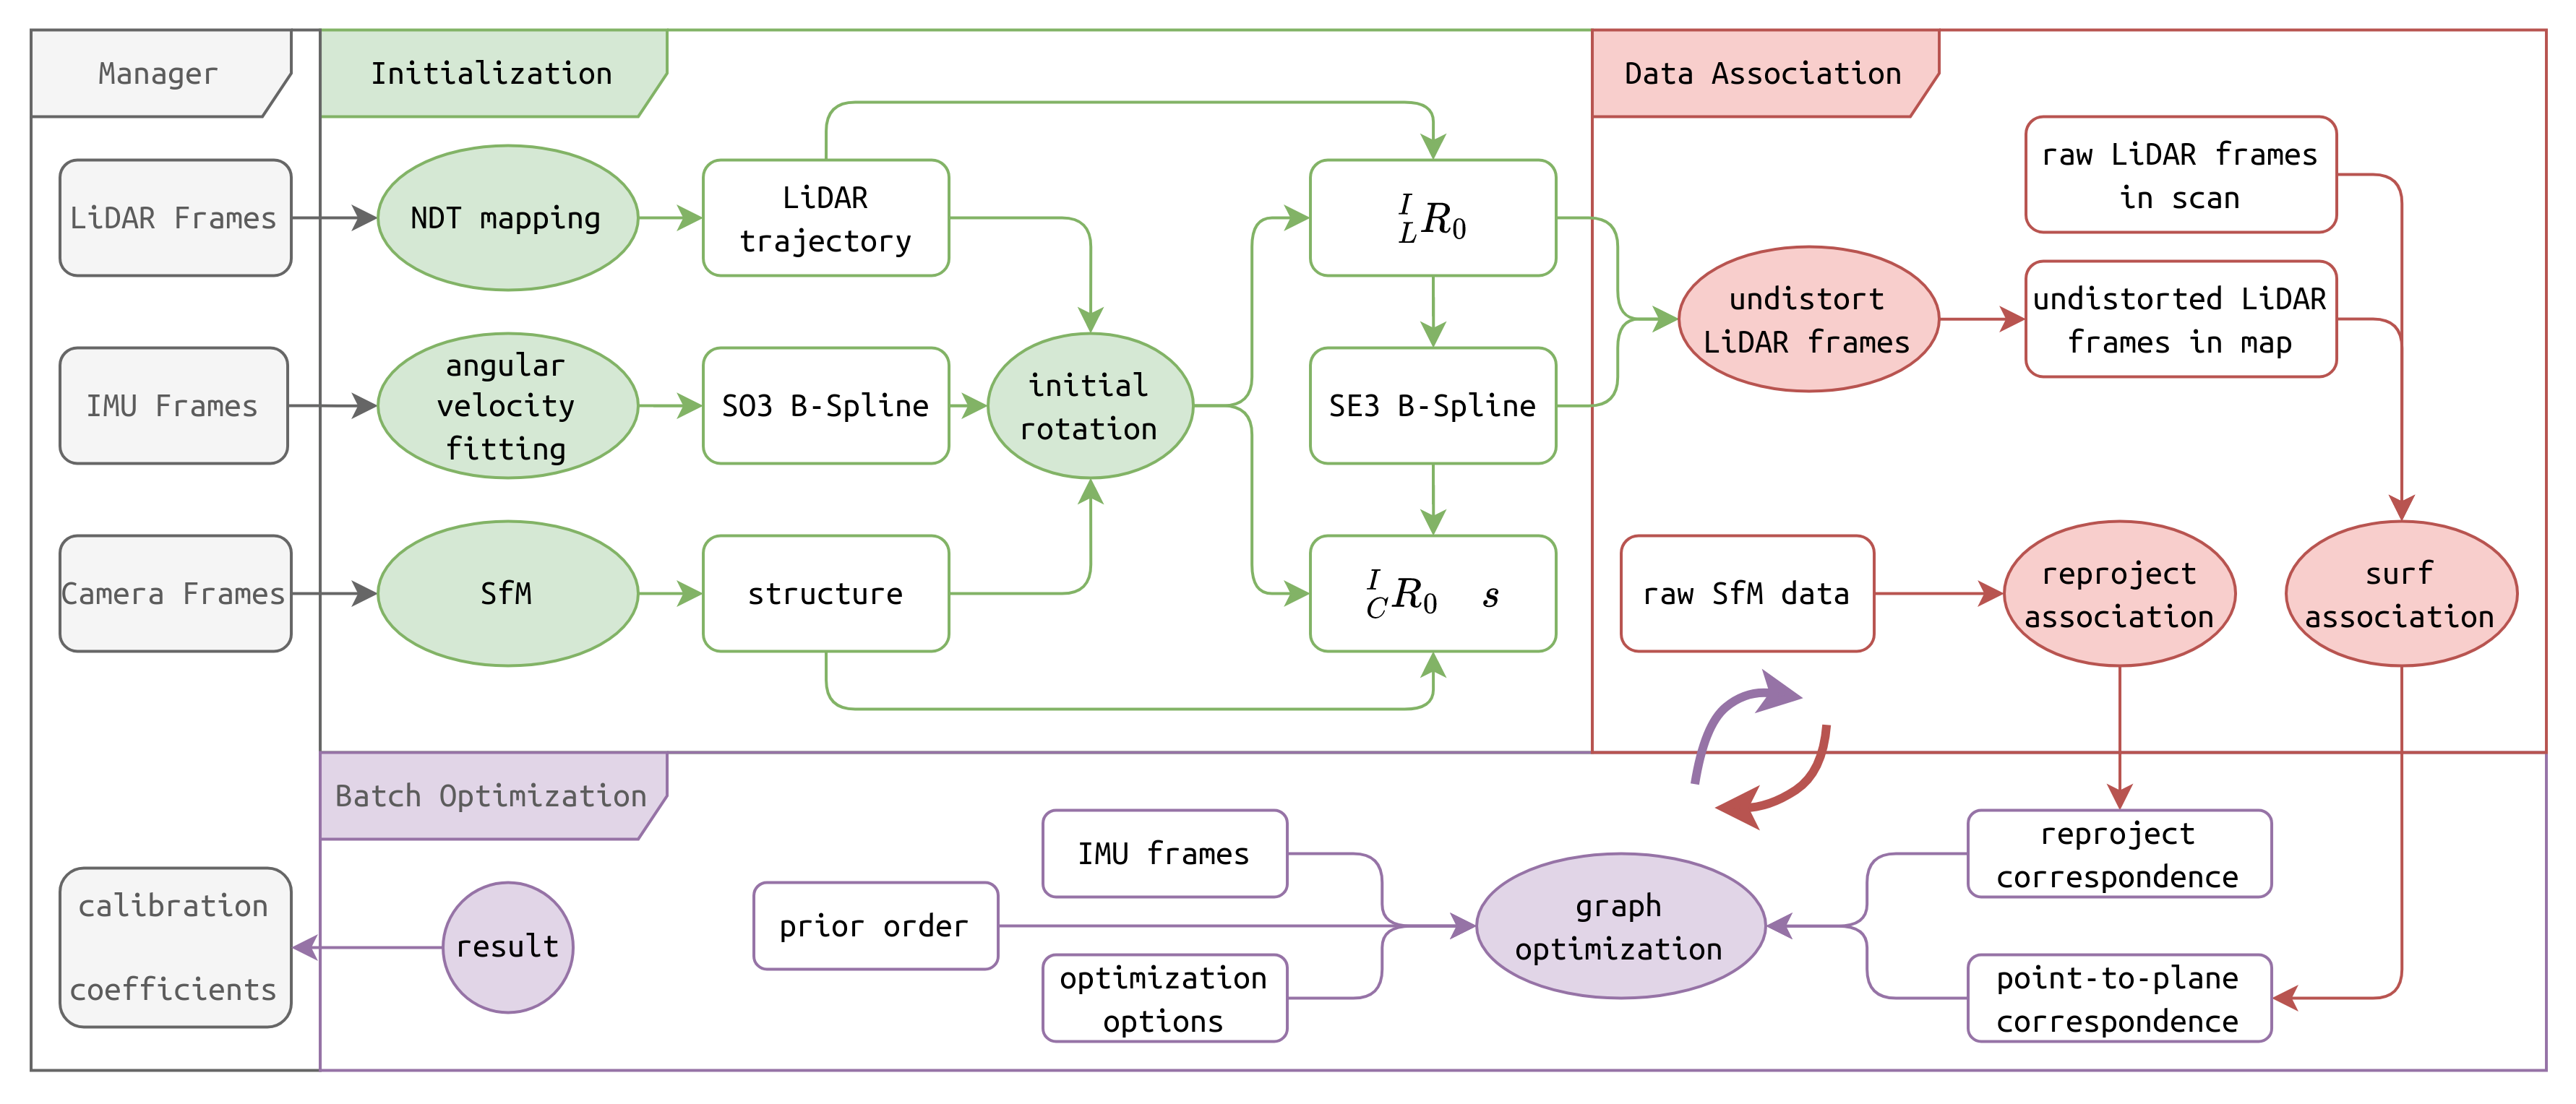
\includegraphics[width=0.9\linewidth]{img/system.png}
    \caption{\normf{基于连续时间的LiDAR/Camera/IMU的时空标定方法流程图}}

    \label{fig:system}
  \end{figure}
}

\label{subsec:state_vector_define}
在\ref{suubsubsec:calib_param}节中,已对待标参数做了简单的分类说明。为后续算法阐述的清晰性和便利性,现对估计优化中涉及的状态作一个完整定义:
\begin{equation}
  \begin{aligned}
    \boldsymbol{x}   & =\left\lbrace
    \boldsymbol{x}_I,\boldsymbol{x}_L,\boldsymbol{x}_C,\boldsymbol{x}_B
    \right\rbrace_{(48+m+6n)\times 1}                                                                                                                                                                      \\
    \boldsymbol{x}_I & =\left\lbrace\boldsymbol{M}_{a},\boldsymbol{b}_a,\boldsymbol{M}_{\omega},\boldsymbol{b}_\omega,{^{G}_{I}\boldsymbol{q}}, {^{I_0}\boldsymbol{g}} \right\rbrace_{23\times 1}          \\
    \boldsymbol{x}_L & =\left\lbrace{^{I}_{L}\boldsymbol{q}},{^{I}}\boldsymbol{p}_{L},{^{I}t_{L}}\right\rbrace_{7\times 1}                                                                                 \\
    \boldsymbol{x}_C & =\left\lbrace {^{I}_{C}\boldsymbol{q}},{^{I}}\boldsymbol{p}_{C},{^{I}t_{C}}\mid\boldsymbol{K},\boldsymbol{d},t_r\mid s,\lambda_0,\cdots,\lambda_{m-1}\right\rbrace_{(18+m)\times 1} \\
    \boldsymbol{x}_B & =\left\lbrace \boldsymbol{q}_0,\boldsymbol{p}_0,\cdots,\boldsymbol{q}_{n-1},\boldsymbol{p}_{n-1}\right\rbrace_{6n\times 1}
  \end{aligned}
\end{equation}
总的状态向量包含4个部分:IMU状态向量$\boldsymbol{x}_I$、LiDAR状态向量$\boldsymbol{x}_L$,Camera状态向量$\boldsymbol{x}_C$和位姿B样条状态向量$\boldsymbol{x}_B$,其含义和\ref{suubsubsec:calib_param}节中所述一致。为了可区分性,在相机状态向量里用符号$\mid$对不同类别状态进行划分,同时将相机的像素焦距、像主点表示为内参矩阵$\boldsymbol{K}$,径向畸变参数和切向畸变表示为$\boldsymbol{d}$。在位姿B样条曲线部分,本文基于的是IMU的位姿轨迹进行构建,因为相较于LiDAR和Camera,IMU的输出频率更高,能保证位姿B样条的精度。

\section{\normf{初始化}}
初始化步骤对于参数估计是重要的。一方面,数据关联为批处理优化构建约束,而构建关联的信息,需要通过初始化来提供(如点到面关联的构建需要基于初始化的LiDAR地图,详细内容见\ref{subsubsec:point_to_plane}节)。另一方面,本文使用的是基于因子图优化的参数估计方法,在给定初值的情况下,通过不断迭代求解,精化待估参数,直至算法收敛。因而一个好的初值对于算法能否收敛,以及收敛速度有较大影响。下面对初始化部分进行阐述。
\subsection{\normf{IMU姿态B样条的初始化}}
从式\ref{equ:imu_bspline}可知,基于已有的位姿B样条曲线,通过时间微分可以得到线加速度和角速度信息。反之,在已知加速度和角速度的条件下,可以通过构建约束,恢复出位姿B样条。由于IMU能够感知惯性系下载体的线加速度和角速度,为恢复出位姿B样条提供了条件。令$\boldsymbol{r}^i(\omega)$、$\boldsymbol{r}^i(a)$分别表示与第$i$个角速度和线加速度帧相关的损失函数,结合式\ref{equ:imu_model},有:
\begin{equation}
  \label{equ:imu_const}
  \begin{cases}
    \begin{aligned}
      \boldsymbol{r}^i(\omega) & =\boldsymbol{M}_\omega\cdot{^{G}_{I}\boldsymbol{R}}\cdot{^{I}}\boldsymbol{\omega}(t_{I_i})+\boldsymbol{b}_\omega+\boldsymbol{n}_\omega-{^{G}}\boldsymbol{\omega}_m(t_{I_i}) \\
      \boldsymbol{r}^i(a)      & =\boldsymbol{M}_a\cdot{^{I}}\boldsymbol{a}(t_{I_i})+\boldsymbol{b}_a+\boldsymbol{n}_a-{^{A}}\boldsymbol{a}_m(t_{I_i})
    \end{aligned}
  \end{cases}
\end{equation}
其中$\boldsymbol{\omega}(t_{I_i})$和$\boldsymbol{a}(t_{I_i})$由式\ref{equ:imu_bspline}计算得到。因此优化问题可表示为:
\begin{equation}
  \min_{\boldsymbol{x}_B} \sum_{i\in\mathcal{I}^\dagger}\left( \Vert\boldsymbol{r}^i(\omega)\Vert^2_{\Sigma_\omega}+\Vert\boldsymbol{r}^i(a)\Vert^2_{\Sigma_a}\right)
\end{equation}
其中:$\Sigma_a$和$\Sigma_\omega$分为线加速度和角速度约束对应的协方差矩阵;运算符$\Vert\boldsymbol{A}\Vert^2_{\boldsymbol{B}}=\boldsymbol{A}^T\boldsymbol{B}^{-1}\boldsymbol{A}$。而后通过高斯-牛顿法(Gauss-Newton,GN)或者列文伯格-马夸尔特法(Levenberg-Marquardt,LM)\footnote{\normf{本文使用LM方法,具体介绍见附录\ref{appendix:lm_alg}。}}等优化方法进行参数求解,具体可参考\cite{barfoot2017state}。

需要注意的是,$I_0$系下表示的重力向量${^{I_0}\boldsymbol{g}}$和加速度耦合在一起(见式\ref{equ:imu_bspline}),在未知${^{I_0}\boldsymbol{g}}$的情况下,无法构建加速度信息对位姿B样条曲线的约束,相应的,也无法得到位姿B样条中的位移信息。因此,在本处只初始化IMU位姿B样条中的姿态曲线,如图\ref{fig:so3_bspline}所示,位移曲线则通过对齐LiDAR位姿序列得到,具体见\ref{subsubsec:init_so3_bspline}节。
%%%%%%%%%%%%%%%%%%%%%%%%%%%%%%%%%%%%%%%%%%%%%%%%%%%%%%%%%%%%%%%%%%%%%%%%%%%%%%%%%%%%%%%%%
\mlcomment{
  \begin{figure}[htbp]
    \centering
    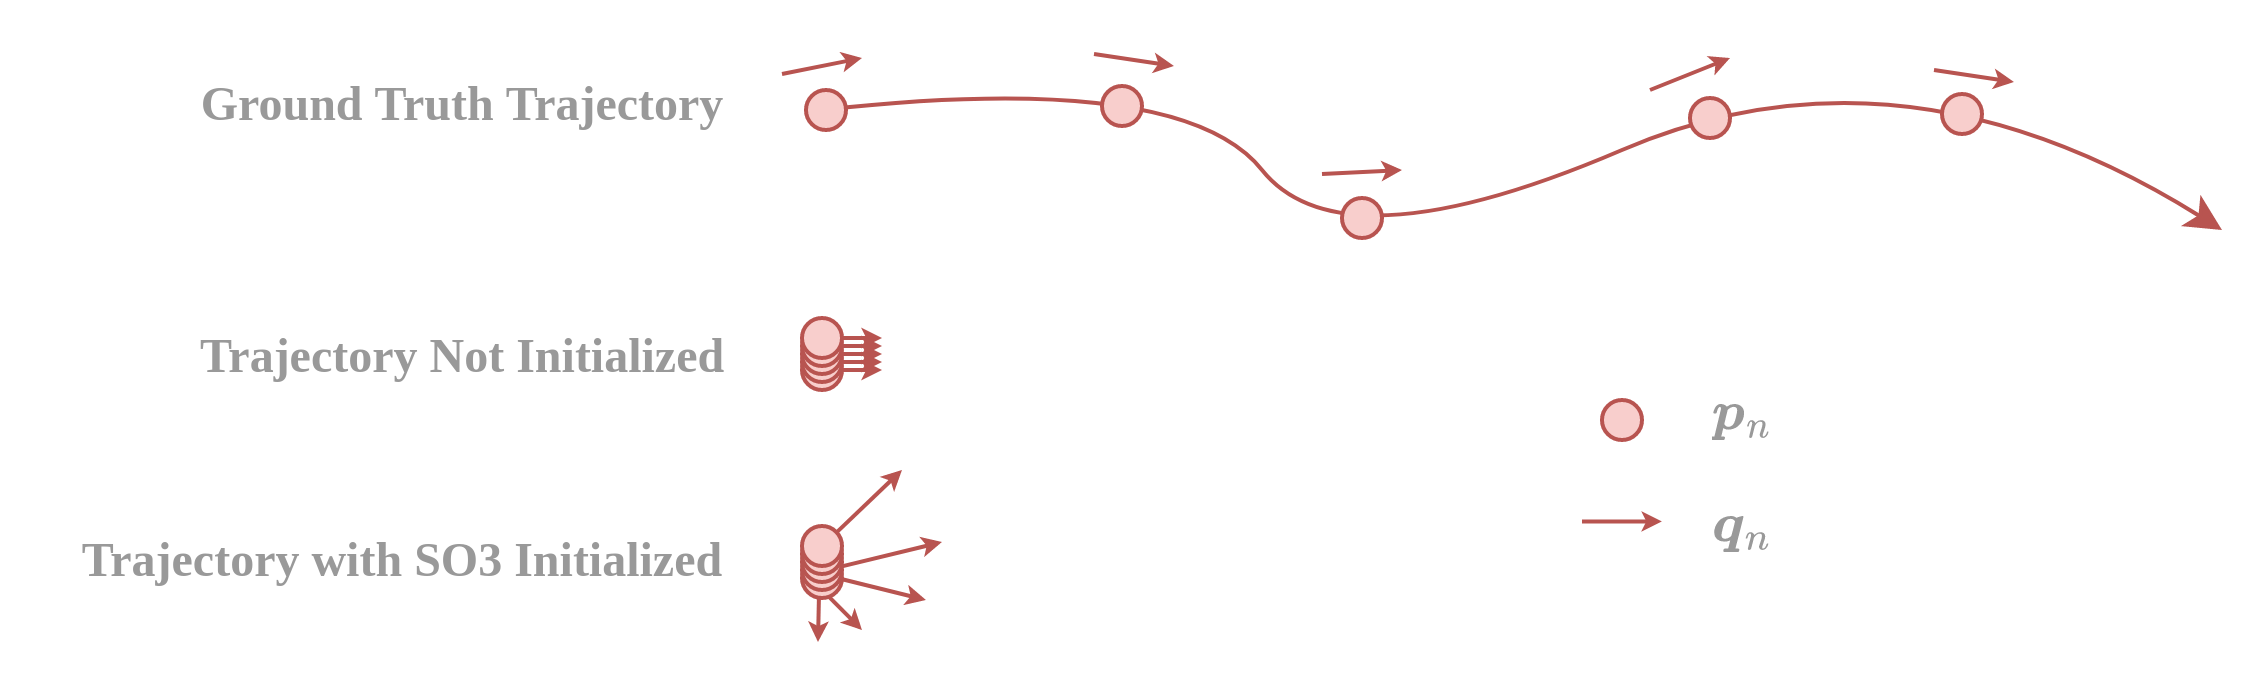
\includegraphics[width=0.9\linewidth]{img/so3_bspline.png}
    \caption{\normf{IMU姿态B样条的初始化}}
    \label{fig:so3_bspline}
  \end{figure}
}

IMU姿态B样条初始化完成后,获得了IMU姿态B样条曲线$\mathcal{B}$,同时可以通过查询获得离散的IMU位姿序列$\mathcal{I}=\left\lbrace {^{I_0}_{I_{i}}}\boldsymbol{T} \right\rbrace,i\in\mathcal{I}^\dagger$。二者用于后续约束的构建和相关参数的初始化。

\subsection{\normf{LiDAR轨迹的初始化}}
初始化LiDAR轨迹的目的在于生成初始点云地图,以进行点到面约束的构建,同时带有尺度信息的LiDAR轨迹可以初始化相机的尺度。本文使用NDT算法(The Normal Distributions Transform)进行LiDAR轨迹的初始化。NDT算法将参考点云帧空间细分为网格,并对每个网格求解正态分布,用来描述测量一个点的概率。对于参考点云帧的某个网格$G_i$内的$m$个点,有:
\begin{equation}
  \begin{aligned}
                        & p(\boldsymbol{x})\propto\exp\left(-\frac{(\boldsymbol{x}-\boldsymbol{\mu}_i)^T\boldsymbol{\Sigma}^{-1}_i(\boldsymbol{x}-\boldsymbol{\mu}_i)}{2}\right)                                                 \\
    \boldsymbol{\mu}_i= & \frac{1}{m}\sum_{j\in(G_i)^\dagger}\boldsymbol{p}_i^j\quad \boldsymbol{\Sigma}_i=\frac{1}{m-1}\sum_{j\in(G_i)^\dagger}(\boldsymbol{p}_i^j-\boldsymbol{\mu}_i)(\boldsymbol{p}_i^j-\boldsymbol{\mu}_i)^T
  \end{aligned}
\end{equation}
对于待对齐帧,基于位姿初值,将其变换到参考帧坐标系下,并计算所有点落在各格网的概率和,作为配准得分。通过优化,当使得配准得分最大时,即可获得对应于该准则下的最优位姿变换参数。与经典的ICP方法\cite{rusinkiewicz2001efficient}相比较,NDT算法不需要对齐点特征,能够直接进行配准和计算,所以在计算时不会消耗过多代价,且概率密度函数计算较为简单,极大的提高了算法的效率 。因此本文使用NDT算法作为点云配准方法。

LiDAR轨迹初始化完成后,获得了点云地图$\mathcal{M}$和离散的LiDAR位姿序列$\mathcal{L}=\left\lbrace {^{L_0}_{L_{i}}}\boldsymbol{T} \right\rbrace,i\in\mathcal{L}^\dagger$。二者用于后续约束的构建和相关参数的初始化。

\subsection{\normf{Camera场景结构的初始化}}
初始化Camera场景结构的目的在于构建重投影约束并初始化路标点的深度信息(具体见\ref{subsubsec:reproject}节)。从约束构建的角度出发,恢复相机场景结构有两类方法:一种是基于图像几何特征进行优化,称之为特征法,如ORB-SLAM\cite{mur2015orb}、VINS-Mono\cite{qin2018vins}等在处理该类问题时使用了特征法;另一种是基于图像灰度域进行优化,称之为直接法,如SVO\cite{forster2014svo}、LSD-SLAM\cite{engel2014lsd}等。直接法存在光强不变假设,但该假设在现实世界中很容易被破坏,导致解算失败。因此本文使用基于特征的方法,利用SfM方法(Structure from motion)进行场景重建。
%%%%%%%%%%%%%%%%%%%%%%%%%%%%%%%%%%%%%%%%%%%%%%%%%%%%%%%%%%%%%%%%%%%%%%%%%%%%%%%%%%%%%%%%%
\mlcomment{
  \begin{figure}[htbp]
    \centering
    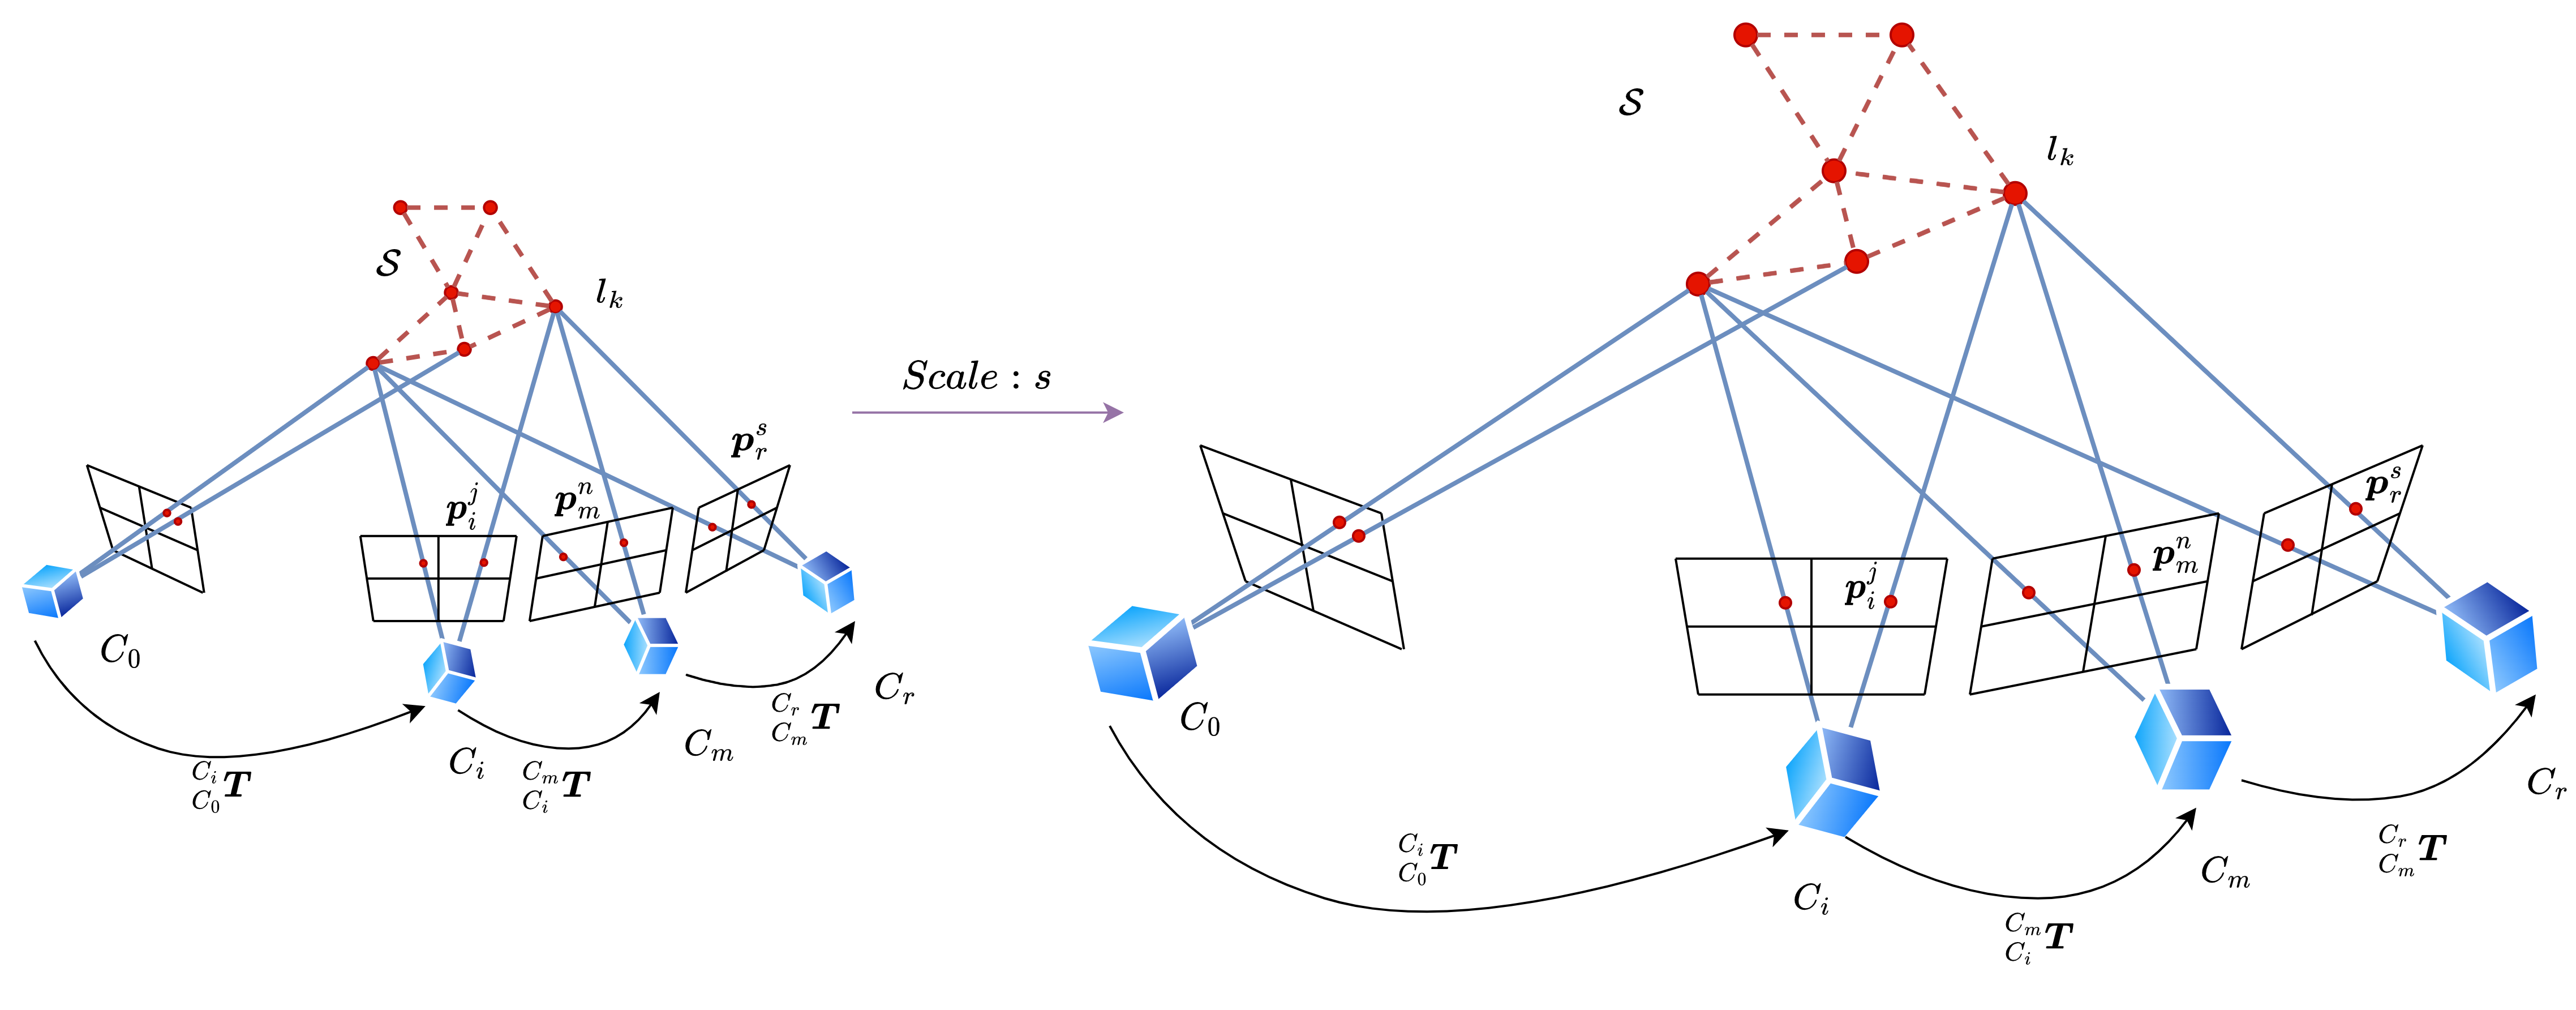
\includegraphics[width=0.95\linewidth]{img/structure.png}
    \caption{\normf{相机场景结构}}
    \label{fig:structure}
  \end{figure}
}

SfM算法一般包含如下的几个步骤:
\begin{enumerate}
  \item 图像特征提取和描述

        图像特征是一组与计算机相关的信息,计算任务取决与具体的应用,是图像信息的另一种数字表达形式\cite{高翔2017视觉}。在本文中,图像特征特指图像中的二维几何信息,如点、线、面等。基于该类几何特征信息,可以通过相应的多视图几何算法,恢复出场景的三维结构。因此在SfM中,一般要对图像特征进行提取,且为了后续的特征匹配,往往还会对所提取的特征进行描述。较为常用的图像几何特征是点特征,如ORB特征\cite{rublee2011orb}、SIFT特征\cite{lowe2004distinctive}等。其中ORB特征计算效率高,具有尺度和旋转不变性;而SIFT特征相较于ORB特征计算效率偏低,但是其对旋转、尺度缩放、亮度变化具有不变性,对视角变化、仿射变换、噪声也有一定程度的稳定性,能够保证提取到的特征在子像素级的精度。由于本文研究的标定方法是一种离线标定算法,对实时性要求不高,因此使用SIFT算法进行特征的提取和描述,以保证算法的精度。

  \item 特征匹配

        相机在成像过程中将三维场景映射到二维像平面上,导致了场景深度信息的缺失,因此单张影像无法恢复出场景的三维信息。但基于多张共视影像之间的特征匹配关系,可以恢复出场景三维信息。特征匹配即基于特征的描述向量(称为描述子),寻找不同共视影像上的同名特征\footnote{\normf{图像上的同名特征指存在于不同共视影像上但对应场景中同一实体的特征集合。}},构建匹配关系。特征匹配本质上是一个模式匹配问题,常用的匹配算法有汉明距离匹配(Hamming Distance Matching)、暴力匹配(Brute-Force Matching)等。
  \item 光束法平差(Bundle Adjustment,BA)

        基于提取到的特征和匹配关系,通过光束法平差,可以恢复出场景的三维结构。在该过程中,根据路标点的参数化方式的不同,约束构建存在两种方法:投影约束和重投影约束。

        投影约束直接在世界参考坐标系下(如$C_0$系)参数化点的三维位置。设点$\boldsymbol{l}_k$为世界坐标系下的一个路标点,其投影到第$i$张影像上的第$j$个特征点$\boldsymbol{p}_i^j$,如图\ref{fig:structure}所示,则有:
        \begin{equation}
          \boldsymbol{p}_i^j=\pi\left( s \cdot{^{C_i}_{W}\boldsymbol{R}}\cdot\boldsymbol{l}_k+{^{C_i}\boldsymbol{p}_{W}}\right) +\boldsymbol{n}_i^j
        \end{equation}
        其中:$\boldsymbol{n}_i^j$为观测噪声;$\pi:\mathbb{R}^3\mapsto\mathbb{R}^2$为投影函数,其将$C_i$系下的三维点投影到像素坐标系上,其具体形式取决于相机的成像模型。本文使用针孔成像模型,投影函数$\pi$的具体形式见式\ref{equ:cam_pinhole}、式\ref{equ:cam_pinhole_dist}。由此,损失函数为:
        \begin{equation}
          \boldsymbol{r}_{ij}^k(c)=\pi\left( s \cdot{^{C_i}_{W}\boldsymbol{R}}\cdot\boldsymbol{l}_k+{^{C_i}\boldsymbol{p}_{W}}\right)+\boldsymbol{n}_i^j-\boldsymbol{p}_i^j
        \end{equation}
        最后,基于投影约束的BA问题可以表述为:
        \begin{equation}
          \min_{\mathcal{C},\mathcal{S}} \sum_{i\in\mathcal{C}^\dagger,j\in\mathcal{F}^\dagger,k\in\mathcal{S}^\dagger}\Vert \boldsymbol{r}_{ij}^k(c)\Vert^2_{\Sigma_c}
        \end{equation}
        其中:$\mathcal{F}$表示特征集合,$\mathcal{S}$表示路标地图,其余符号含义与前文所述保持一致。注意到,在优化问题中,优化的状态为相机位姿序列$\mathcal{C}$和路标地图$\mathcal{S}$,同时上式显式的将尺度信息$s$包含了进来。

        而重投影约束则在参考相机帧(如第一次观察到路标点的相机帧)坐标系下,结合深度信息参数化路标点。设世界坐标系下的路标点$\boldsymbol{l}_k$在第$i$个相机帧被首次观察到,并投影为第$j$个特征点$\boldsymbol{p}_i^j$,而后又被第$m$个相机帧观察到,并投影为第$n$个特征点$\boldsymbol{p}_m^n$,如图\ref{fig:structure}所示,则有:
        \begin{equation}
          \boldsymbol{p}_m^n=\pi\left({^{C_m}_{C_i}\boldsymbol{T}}\cdot \pi^{-1}\left(\boldsymbol{p}_i^j,\lambda_i^j\right)\right) +\boldsymbol{n}_m^n
        \end{equation}
        其中$\pi^{-1}:\mathbb{R}^2\mapsto\mathbb{R}^3$为反投影函数。与投影函数$\pi$不同,反投影函数$\pi^{-1}$基于额外输入的深度信息,将像素平面上的二维点投影到三维相机坐标系下。本文使用逆深度$\lambda=1/d$表示深度信息,以保证噪声的高斯特性\cite{montiel2006unified}。由此,损失函数为:
        \begin{equation}
          \label{equ:reproject}
          \boldsymbol{r}_{ij}^{mn}(c)=\pi\left({^{C_m}_{C_i}\boldsymbol{T}}\cdot s \cdot\pi^{-1}\left(\boldsymbol{p}_i^j,\lambda_i^j\right)\right) +\boldsymbol{n}_m^n-\boldsymbol{p}_m^n \\
        \end{equation}
        最后,基于重投影约束的BA问题可以表述为:
        \begin{equation}
          \min_{\mathcal{C},\mathcal{S}} \sum_{i,m\in\mathcal{C}^\dagger,j,n\in\mathcal{F}^\dagger}\Vert \boldsymbol{r}_{ij}^{mn}(c)\Vert^2_{\Sigma_c}
        \end{equation}
        注意到,虽然在目标函数中没有将路标地图$\mathcal{S}$显式表达出来,但是求解路标点逆深度的过程等价于求解路标地图。

        无论是基于投影约束的BA还是基于重投影约束的BA,本质上没有区别。在涉及到BA问题时,约束的构建视具体情况而选择,如ORB-SLAM\cite{mur2015orb}在世界参考坐标系下参数化路标点,使用的是基于投影约束的BA;而VINS-Mono\cite{qin2018vins}则使用的是基于重投影约束的BA。本文使用基于重投影约束的BA。

\end{enumerate}
相机场景结构初始化完成后,获得了路标地图(场景结构)$\mathcal{S}$和离散的相机位姿序列$\mathcal{C}=\left\lbrace {^{C_0}_{C_{i}}}\boldsymbol{T} \right\rbrace,i\in\mathcal{C}^\dagger$。二者用于后续约束的构建和相关参数的初始化。

\subsection{\normf{外参和相机尺度的初始化}}
对于图优化而言,良好的参数初值至关重要。在参数初始化部分,本文主要考虑了外参的初始化以及相机场景结构尺度因子的初始化,因为二者是否被正确初始化对于批处理优化影响较大,不合理的初值会导致解算失败。

在外参的初始化上,本文使用经典的手眼标定法(Hand-eye),通过对齐两个位姿序列求解外参。以IMU和Camera外参的初始化为例,具体如图\ref{fig:hand_eye}所示。基于初始化的IMU位姿B样条$\mathcal{B}$和Camera位姿序列$\mathcal{C}$,对每一个相邻的相机位姿对$C_k$和$C_{k+1}$,有如下的等式:
\begin{equation}
  \label{equ:hand_eye}
  \begin{aligned}
    {{^{I}_{C}}\boldsymbol{T}}\cdot{^{C_k}_{C_{k+1}}\boldsymbol{T}}                                                                                                                                                                                                            & ={^{I_k}_{I_{k+1}}\boldsymbol{T}}\cdot{{^{I}_{C}}\boldsymbol{T}} \\\to
    \begin{pmatrix}
      {{^{I}_{C}}\boldsymbol{q}}\circ{^{C_k}_{C_{k+1}}\boldsymbol{q}} & {{^{I}_{C}}\boldsymbol{q}}\circ{^{C_k}\boldsymbol{p}_{C_{k+1}}}+{^{I}\boldsymbol{p}_{C}} \\
      \boldsymbol{0}                                                  & 1
    \end{pmatrix} & =\begin{pmatrix}
                       {{^{I_k}_{I_{k+1}}}\boldsymbol{q}}\circ{^{I}_{C}\boldsymbol{q}} & {{^{I_k}_{I_{k+1}}}\boldsymbol{q}}\circ{^{I}\boldsymbol{p}_{C}}+{^{I_k}\boldsymbol{p}_{I_{k+1}}} \\
                       \boldsymbol{0}                                                  & 1
                     \end{pmatrix}
  \end{aligned}
\end{equation}
基于该约束可以求解IMU与Camera之间的外参。
%%%%%%%%%%%%%%%%%%%%%%%%%%%%%%%%%%%%%%%%%%%%%%%%%%%%%%%%%%%%%%%%%%%%%%%%%%%%%%%%%%%%%%%%%
\mlcomment{
  \begin{figure}[htbp]
    \centering
    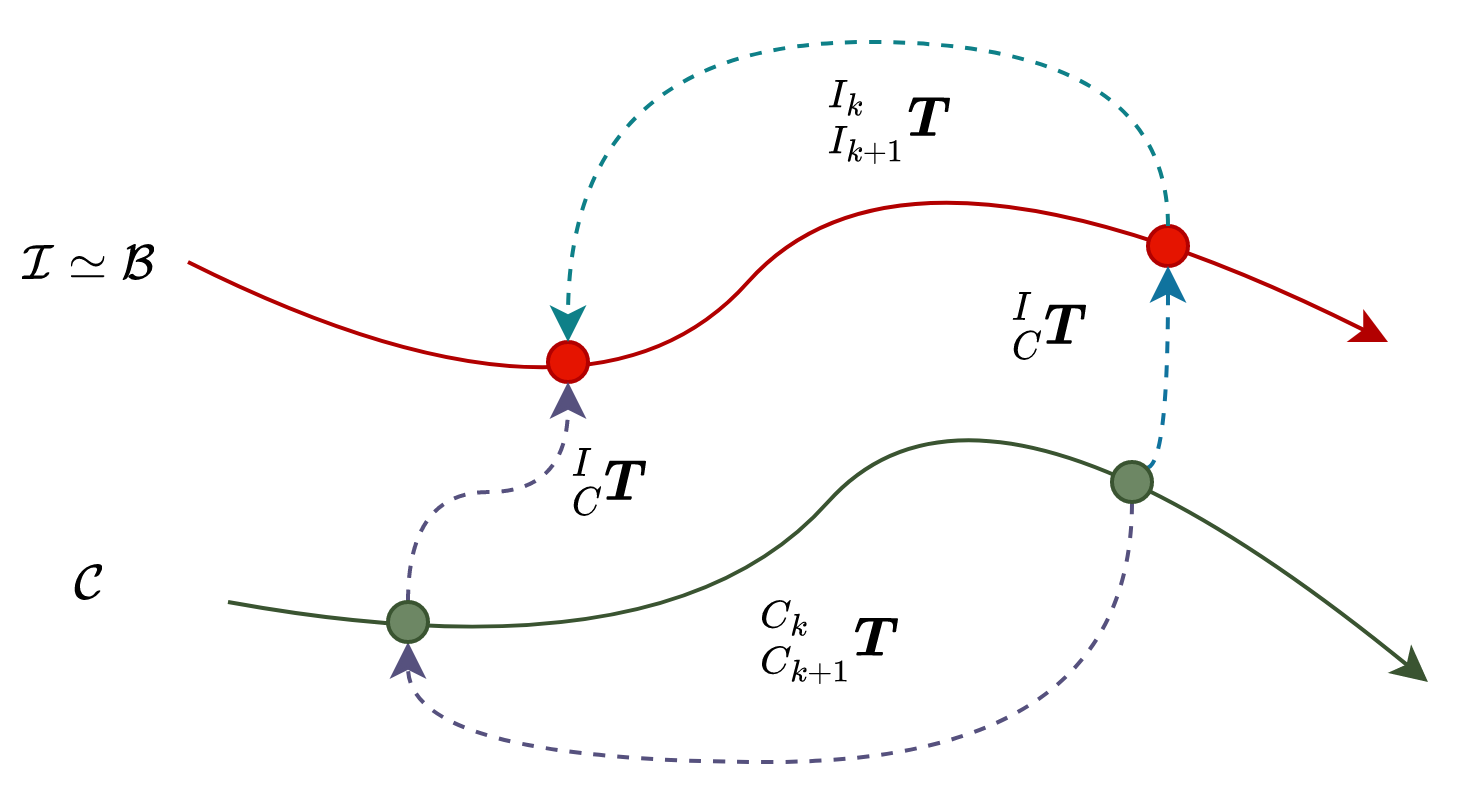
\includegraphics[width=0.5\linewidth]{img/hand_eye.png}
    \caption{\normf{IMU和Camera外参的初始化}}
    \label{fig:hand_eye}
  \end{figure}
}

\label{subsubsec:init_extri_pos}
在初始化IMU位姿B样条时,由于重力向量和加速度耦合在一起,因此只初始化了IMU位姿B样条中的姿态曲线。所以在初始化外参时,本文选择只初始化姿态量,位移量直接初始化为零向量$\boldsymbol{0}_{3\times 1}$,该种简单处理对结果造成的影响有限(只会对批处理优化阶段的迭代次数有些许影响)。只考虑式\ref{equ:hand_eye}中的姿态等式,有:
\begin{equation}
  {{^{I}_{C}}\boldsymbol{q}}\circ{^{C_k}_{C_{k+1}}\boldsymbol{q}}={{^{I_k}_{I_{k+1}}}\boldsymbol{q}}\circ{^{I}_{C}\boldsymbol{q}}
\end{equation}
为方便求解,将四元数乘法写为矩阵乘法并化简,有:
\begin{equation}
  \label{equ:relative_rot}
  \left(\boldsymbol{M}^*\left({^{C_k}_{C_{k+1}}\boldsymbol{q}}\right)-\boldsymbol{M}\left({{^{I_k}_{I_{k+1}}}\boldsymbol{q}}\right)\right)\cdot{^{I}_{C}\boldsymbol{q}}=\boldsymbol{0}_{4\times 4}
\end{equation}
其中$\boldsymbol{M}^*(\cdot)$和$\boldsymbol{M}(\cdot)$的含义为:对于四元数$\boldsymbol{q}=\begin{pmatrix}	q_w&q_x&q_y&q_z	\end{pmatrix}^T=\begin{pmatrix}	q_w&\boldsymbol{q}_v^T	\end{pmatrix}^T$,有:
\begin{equation*}
  \boldsymbol{M}(\boldsymbol{q})=\begin{pmatrix}
    q_w              & -\boldsymbol{q}_v^T                                          \\
    \boldsymbol{q}_v & q_w\cdot\boldsymbol{I}_{3\times 3}+\liehat{\boldsymbol{q}_v}
  \end{pmatrix}\quad
  \boldsymbol{M}^*(\boldsymbol{q})=\begin{pmatrix}
    q_w              & -\boldsymbol{q}_v^T                                          \\
    \boldsymbol{q}_v & q_w\cdot\boldsymbol{I}_{3\times 3}-\liehat{\boldsymbol{q}_v}
  \end{pmatrix}
\end{equation*}
记式\ref{equ:relative_rot}为:${^{k}_{k+1}\boldsymbol{A}}\cdot{^{I}_{C}\boldsymbol{q}}=\boldsymbol{0}$。基于相机姿态序列,可以构建方程$\boldsymbol{A}\boldsymbol{x}=\boldsymbol{0}$。使用SVD方法\cite{barfoot2017state}分解系数矩阵$\boldsymbol{A}$,则最小特征值对应的特征向量即为方程的解。注意,在SVD分解过程中存在参数向量模长为1的约束,能够保证求解得到的四元数是在流形空间$S^3$上的单位四元数(旋转四元数)。IMU和LiDAR外参初始化过程同IMU和Camera外参初始化过程。

\label{subsubsec:init_so3_bspline}
初始化IMU和LiDAR之间的旋转量后,就可以基于带有尺度的LiDAR位姿序列$\mathcal{L}$初始化IMU位姿B样条中的位移量和相机场景尺度因子。对于第$i$个LiDAR位姿${{^{L_0}_{L_i}}\boldsymbol{T}}$,有:
\begin{equation}
  \label{equ:lidar_imu}
  {{^{L_0}_{L_i}}\boldsymbol{T}}={{^{I}_{L}}\boldsymbol{T}^{-1}}\cdot{{^{I_0}_{I}}\boldsymbol{T}^{-1}\left( t_{L_0}+{^{I}t_L}\right) }\cdot{{^{I_0}_{I}}\boldsymbol{T}\left( t_{L_i}+{^{I}t_L}\right) }\cdot{{^{I}_{L}}\boldsymbol{T}}
\end{equation}
其中${{^{I_0}_{I}}\boldsymbol{T}(t)}$可以通过IMU位姿B样条曲线查询获取。基于此,损失函数为:
\begin{equation}
  \boldsymbol{r}^i(l)=\mathrm{Log}\left( {{^{L_0}_{L_i}}\boldsymbol{T}^{-1}}\cdot{{^{I}_{L}}\boldsymbol{T}^{-1}}\cdot{{^{I_0}_{I}}\boldsymbol{T}^{-1}\left( t_{L_0}+{^{I}t_L}\right) }\cdot{{^{I_0}_{I}}\boldsymbol{T}\left( t_{L_i}+{^{I}t_L}\right) }\cdot{{^{I}_{L}}\boldsymbol{T}}\right)
\end{equation}
其中$\mathrm{Log}(\cdot)$为SE(3)上的对数映射,其将SE(3)上的变换矩阵直接映射为李代数$\mathfrak{se}(3)$向量空间中的6维向量。对于Camera位姿序列$\mathcal{C}$而言,同样可以建立如式\ref{equ:lidar_imu}形式的关系。对于第$i$个Camera位姿${{^{C_0}_{C}}\boldsymbol{T}(t_{C_i})}$,同时考虑尺度因子$s$,有:
\begin{equation}
  \label{equ:camera_imu}
  {{^{C_0}_{C_i}}\boldsymbol{T}}\cdot\boldsymbol{S}
  ={{^{I}_{C}}\boldsymbol{T}^{-1}}\cdot{{^{I_0}_{I}}\boldsymbol{T}^{-1}\left( t_{C_0}+{^{I}t_C}\right) }\cdot{{^{I_0}_{I}}\boldsymbol{T}\left( t_{C_i}+{^{I}t_C}\right) }\cdot{{^{I}_{C}}\boldsymbol{T}}\quad \boldsymbol{S}=\begin{pmatrix}
    \boldsymbol{I}_{3} & 0 \\0&s
  \end{pmatrix}
\end{equation}
相应的损失函数为:
\begin{equation}
  \boldsymbol{r}^i(c)=\mathrm{Log}\left(\left( {{^{C_0}_{C_i}}\boldsymbol{T}}\cdot\boldsymbol{S}\right) ^{-1}\cdot {{^{I}_{C}}\boldsymbol{T}^{-1}}\cdot{{^{I_0}_{I}}\boldsymbol{T}^{-1}\left( t_{C_0}+{^{I}t_C}\right) }\cdot{{^{I_0}_{I}}\boldsymbol{T}\left( t_{C_i}+{^{I}t_C}\right) }\cdot{{^{I}_{C}}\boldsymbol{T}} \right)
\end{equation}
最后,优化问题定义为:
\begin{equation}
  \min_{s,\mathcal{B}}\left\lbrace \sum_{i\in\mathcal{L}^\dagger}\Vert\boldsymbol{r}^i(l)\Vert^2_{\Sigma_l}+\sum_{i\in\mathcal{C}^\dagger}\Vert\boldsymbol{r}^i(c)\Vert^2_{\Sigma_c} \right\rbrace
\end{equation}
通过求解这个优化问题,可以完成IMU位姿B样条曲线$\mathcal{B}$和尺度因子$s$的初始化。
\subsection{\normf{其余参数的初始化}}
对于除外参以外的其余待标参数,则直接根据理想的传感器模型进行假定。如加速度计和陀螺仪的零偏$\boldsymbol{b}_\omega$、$\boldsymbol{b}_a$直接初始化为$\boldsymbol{0}_{3\times 1}$,加速度计和陀螺仪的比例因子和交轴耦合误差矩阵$\boldsymbol{M}_{a}$、$\boldsymbol{M}_{\omega}$直接初始化为$\boldsymbol{I}_3$。

而对于相机的内参而言,本文采取的是一种由粗到细的精化方式,需要通过手动给初值的方式进行初始化。原因在于,一方面,当前的相机内参标定方法已经非常成熟,能够通过简单的标定操作获取较高的精度;另一方面,如果在本文的标定框架中对相机内参进行全标定,那么其像素焦距的标定会是一个棘手的问题。针对该问题,在多传感器联合标定中(如相机和LiDAR联合标定),一般通过深度学习或者点云几何特征提取方法\cite{yuan2021pixel},将图像信息关联到真实世界中的实体来构建虚拟靶标,最后构造约束求解。这已超出本文的研究范围,故相机的内参,特别是像素焦距,是通过手动给初值的方式进行初始化的。

\section{\normf{数据关联}}
通过上文的初始化工作,除获得了传感器的离散位姿序列$\mathcal{I}$、$\mathcal{L}$、$\mathcal{C}$,IMU时间连续位姿B样条曲线$\mathcal{B}$以及参数初值外,同时得到了LiDAR点云地图$\mathcal{M}$和相机的场景结构$\mathcal{S}$。基于$\mathcal{M}$和$\mathcal{S}$可以分别构建点到面(point-to-scan)数据关联和重投影(reproject)数据关联。下面对这两个部分进行阐述。

\subsection{\normf{点到面数据关联}}
\label{subsubsec:point_to_plane}
基于LiDAR地图$\mathcal{M}$,可以构建相应的几何关联,如点到点、点到线、点到面等,本文使用的是点到面关联。一方面,在大部分场景中,点云面特征相较于点特征或线特征,是一种较稳健的特征,能够提供较强的约束;另一方面,在LiDAR轨迹初始化过程中使用的是NDT算法,其将点云空间划分为格网,为面特征的提取提供了便利。下面对点到面数据关联的构建过程进行说明。

在构建点到面数据关联时,首先会基于已有的IMU位姿B样条曲线$\mathcal{B}$,对LiDAR帧进行去畸变操作,以将单个LiDAR帧中的异步量测点对齐到同一坐标系下。对于第$i$个LiDAR帧中的第$j$个点$\boldsymbol{p}_j^i$,可以基于IMU和LiDAR的外参信息以及IMU位姿B样条曲线$\mathcal{B}$,将其对齐到LiDAR帧时间撮$t_{L_i}$对应的坐标系下:
\begin{equation}
  \begin{pmatrix}
    {^{L_i}}\boldsymbol{p}_j \\b
  \end{pmatrix}	={{^{I}_{L}}\boldsymbol{T}^{-1}}\cdot{{^{I_0}_{I}}\boldsymbol{T}^{-1}\left( t_{L_i}+{^{I}t_L}\right) }\cdot{{^{I_0}_{I}}\boldsymbol{T}\left( t_{L}(\boldsymbol{p}_j^i)+{^{I}t_L}\right) }\cdot{{^{I}_{L}}\boldsymbol{T}}\cdot		\begin{pmatrix}
    \boldsymbol{p}_j^i \\b
  \end{pmatrix}
\end{equation}
其中:$t_{L}(\boldsymbol{p}_j^i)$表示点$\boldsymbol{p}_j^i$在LiDAR时间系统下的时间撮;$b=\left\lbrace 0,1\right\rbrace $用来表征在去畸变时是否考虑位移量:当$b=0$时,去畸变时只考虑姿态,而$b=1$时,姿态量和位移量都会被考虑。在首次进行LiDAR帧去畸变时\footnote{\normf{数据关联在迭代优化过程中会被多次执行,因此这里的首次去畸变指第一次进行数据关联时的去畸变操作。}},IMU和LiDAR外参中的位移量只被简单的初始化为$\boldsymbol{0}_{3\times 1}$,因而此处去畸变不考虑位移量。而在后面多次批处理优化阶段,IMU和LiDAR外参中的位移量已被估计,这时去畸变会同时考虑姿态量和位移量。

基于去畸变后的LiDAR帧,本文会再次进行NDT算法,以构建更为精确的LiDAR点云地图$\mathcal{M}$。而后基于NDT算法划分的格网,使用RANSAC方法\cite{barfoot2017state}对各格网内的点进行面的拟合,接着通过以下的指标对平面拟合结果进行判定:
\begin{equation}
  p=2\times\frac{\lambda_1-\lambda_0}{\lambda_0+\lambda_1+\lambda_2}
\end{equation}
其中:$\lambda_0$、$\lambda_1$、$\lambda_2$为拟合平面时的内符合点(Inliers)方差矩阵的三个特征值,取值从小到大。当$p$越接近1,就代表拟合的平面越优。通过设定相应的阈值,可以过滤掉大部分的假平面。

最后,基于IMU位姿B样条曲线$\mathcal{B}$,将原始多帧LiDAR数据中的所有点变换到点云地图$\mathcal{M}$的坐标系下。设点$\boldsymbol{p}_j^k\in\mathcal{L}_j$为第$j$个原始LiDAR帧中的第$k$个点,将其变换到$\mathcal{M}$对应的坐标系下,得到点${\boldsymbol{p}_j^k}^\prime$,如图\ref{fig:point_to_plane}所示。设${\boldsymbol{p}_j^k}^\prime$所在的格网存在平面$\boldsymbol{e}_i\in\mathcal{E}$,计算点到平面的距离$g_{ij}^k$:
\begin{equation}
  g_{ij}^k=\boldsymbol{e}_i^T\cdot\begin{pmatrix}
    {\boldsymbol{p}_j^k}^\prime \\1
  \end{pmatrix}
  \quad \mathrm{s.t.}\quad\begin{cases}
    \begin{aligned}
      \boldsymbol{e}_i= & \begin{pmatrix}
                            \boldsymbol{n}_i^T & d_i
                          \end{pmatrix}^T \\
      \boldsymbol{n}_i= & \begin{pmatrix}
                            a_i & b_i & c_i
                          \end{pmatrix}^T
      \quad \boldsymbol{n}_i^T\cdot\boldsymbol{n}_i=1
    \end{aligned}
  \end{cases}
\end{equation}
当$g_{ij}^k$小于一定值时,将点$\boldsymbol{p}_j^k$和平面$\boldsymbol{e}_i$进行关联。最终的关联结果表示为:
\begin{equation}
  \mathcal{D}_{L}=\left\lbrace\mathcal{D}_{\boldsymbol{e}_i} \right\rbrace\quad\mathcal{D}_{\boldsymbol{e}_i}=\left\lbrace \boldsymbol{e}_i\mid\boldsymbol{p}_j^k,\cdots\right\rbrace \quad i\in\mathcal{E}^\dagger
  ,j\in\mathcal{L}^\dagger,k\in(\mathcal{L}_j)^\dagger
\end{equation}
%%%%%%%%%%%%%%%%%%%%%%%%%%%%%%%%%%%%%%%%%%%%%%%%%%%%%%%%%%%%%%%%%%%%%%%%%%%%%%%%%%%%%%%%%
\mlcomment{
  \begin{figure}[htbp]
    \centering
    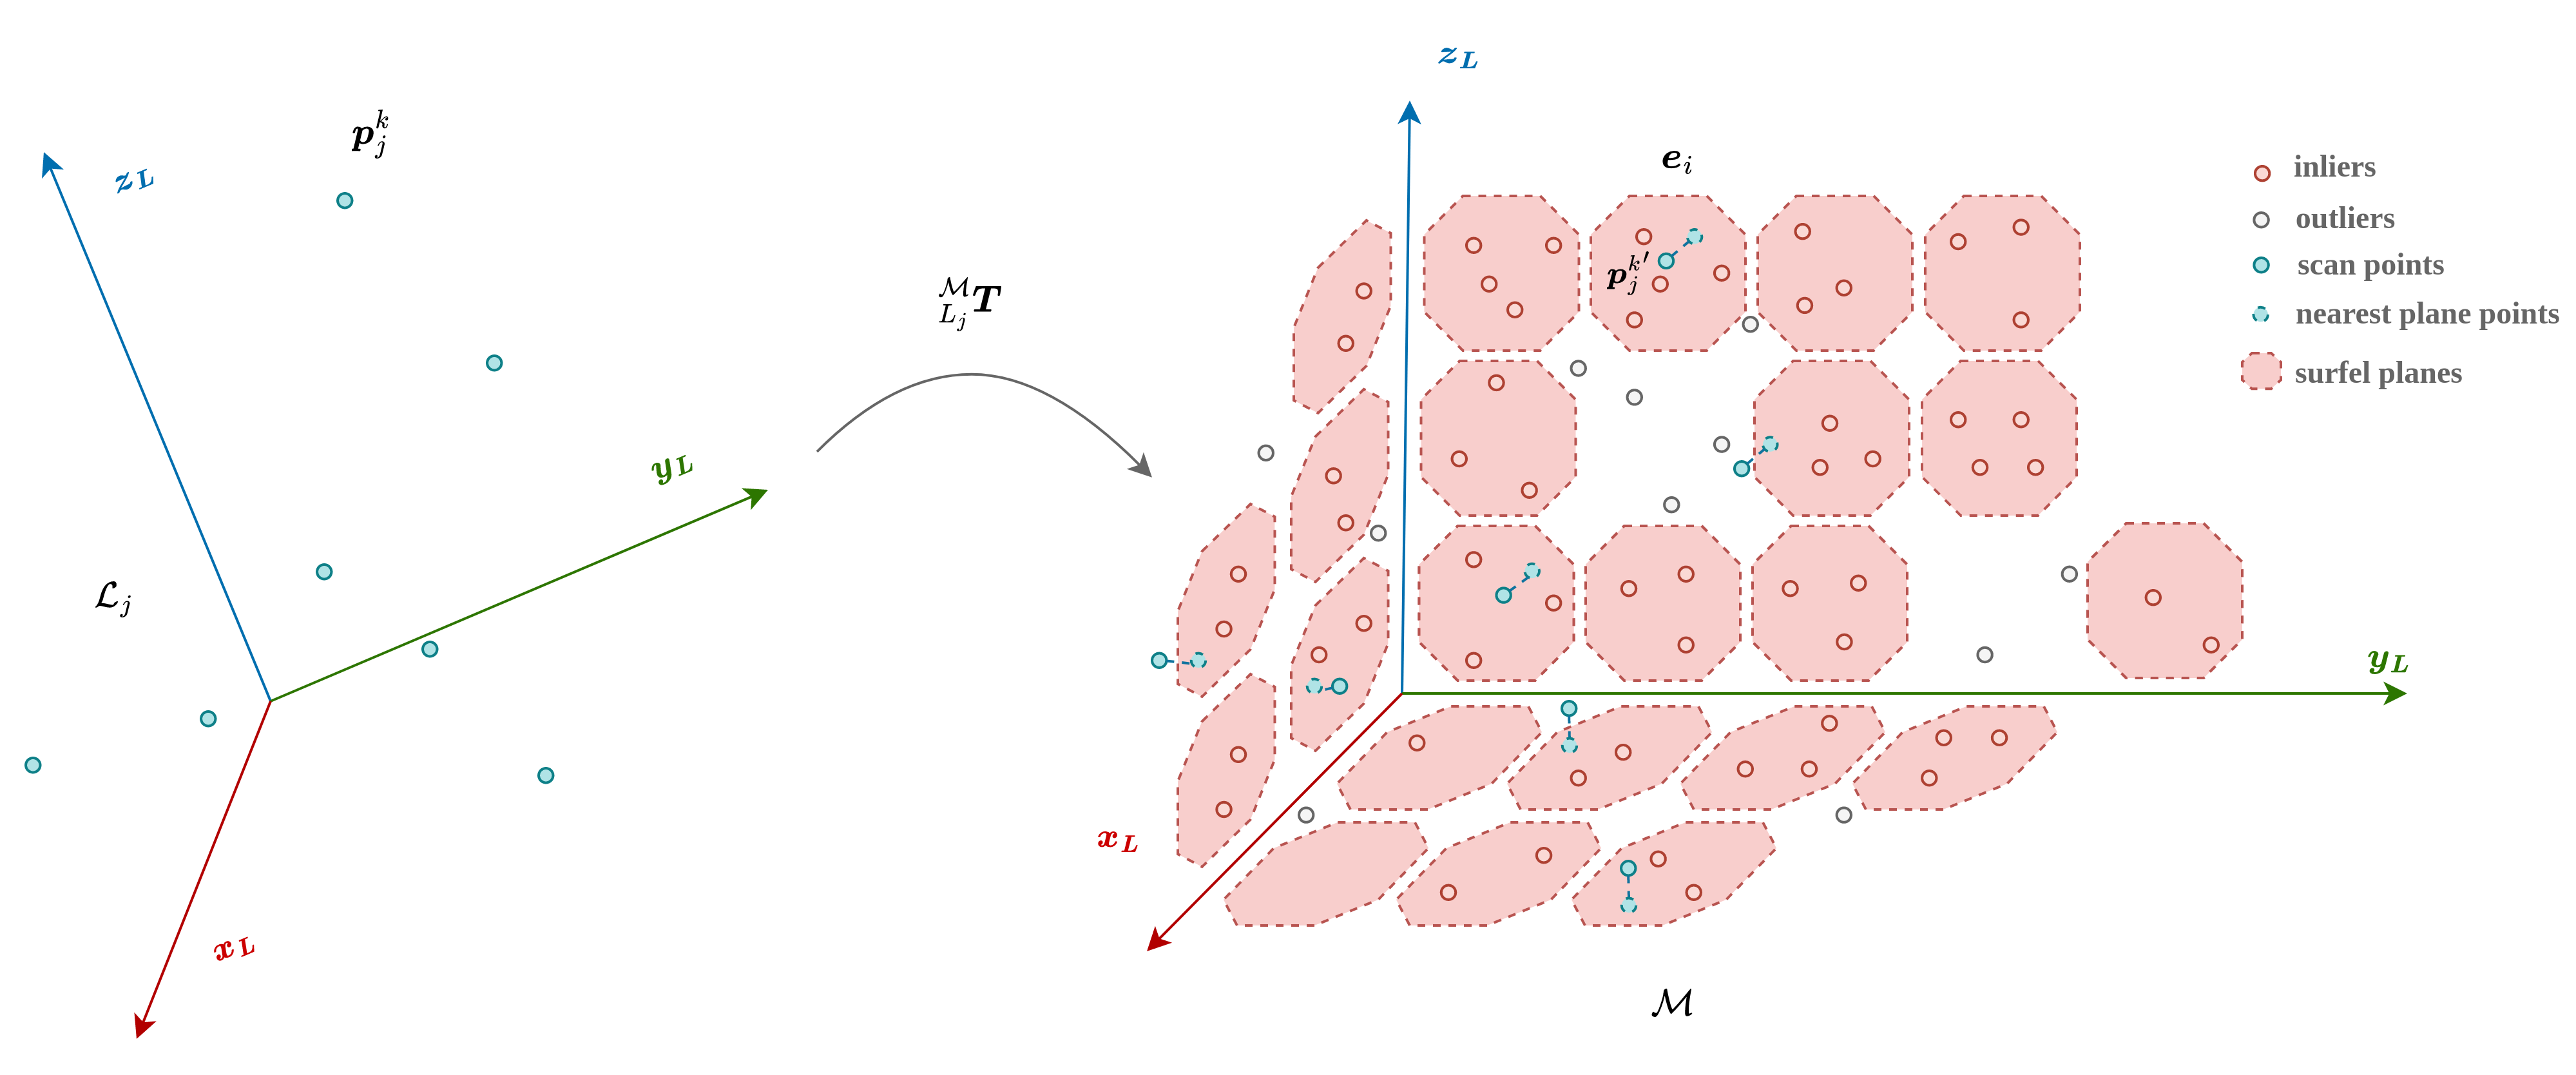
\includegraphics[width=0.9\linewidth]{img/point_to_plane.png}
    \caption{\normf{点到面数据关联过程示意图}}
    \label{fig:point_to_plane}
  \end{figure}
}

\subsection{\normf{重投影数据关联}}
\label{subsubsec:reproject}
基于相机场景结构$\mathcal{S}$,可以进行重投影数据关联的构建,该过程相较于点到面数据关联的构建更简单。设路标$\boldsymbol{l}_k\in\mathcal{S}$依次被相机$C_i$、$C_m$、$C_r\in\mathcal{C}$捕捉,对应的特征点为$\boldsymbol{p}_i^j$、$\boldsymbol{p}_m^n$、$\boldsymbol{p}_r^s\in\mathcal{F}$,如图\ref{fig:structure}所示。则首先在相机$C_i$下使用逆深度$\lambda_i^j$参数化特征点$\boldsymbol{p}_i^j$对应的深度信息,而后构建相机$C_i$与其余观察到路标$\boldsymbol{l}_k$的相机帧$C_m$、$C_r$之间的关联。相应的关联结果表示为:
\begin{equation}
  \mathcal{D}_{C}=\left\lbrace\mathcal{D}_{\boldsymbol{l}_k} \right\rbrace \quad\mathcal{D}_{\boldsymbol{l}_k}=\left\lbrace \boldsymbol{l}_k,\boldsymbol{p}_i^j,\lambda_i^j\mid\boldsymbol{p}_m^n,\boldsymbol{p}_r^s,\cdots\right\rbrace \quad k\in\mathcal{S}^\dagger,i,m,r\in\mathcal{C}^\dagger,j,n,s\in\mathcal{F}^\dagger
\end{equation}

\section{\normf{批处理优化}}
\label{sect:batch_optimization}
基于IMU离散量测数据
$\mathcal{D}_I=\left\lbrace {^{G}}\boldsymbol{\omega}_m^i,\cdots\mid{^{A}}\boldsymbol{a}_m^i,\cdots\right\rbrace,i\in\mathcal{I}^\dagger$
,以及构建的点到面关联$\mathcal{D}_{L}$、重投影关联$\mathcal{D}_{C}$,可以基于因子图优化理论(见\ref{subsec:factor_graph}节)对标定问题进行建模。而后基于构建的因子图进行迭代求解,即可获得因子图中的变量节点的最优估计。本文提出的基于连续时间的LiDAR/Camera/IMU的时空标定方法可建模成如图\ref{fig:problem_model}所示的因子图。图中的圆形或圆角矩形表示待优化的状态变量,含义与\ref{subsec:state_vector_define}节保持一致;矩形或多边形表示因子;实线表示约束。以下对涉及的4种因子进行阐述:
\begin{enumerate}
  \item IMU量测因子

        如前文所述,由于IMU位姿B样条曲线$\mathcal{B}$是时间连续的,对其进行时间微分,可以得到时间连续的线加速度和角速度(见式\ref{equ:imu_bspline}),结合IMU直接提供的离散线加速度和角速度信息,可以构建IMU量测因子,具体的损失函数已在式\ref{equ:imu_const}中给出。注意到,在该因子中,将和IMU相关的状态参量$\boldsymbol{x}_I$纳入到了因子图中,同时涉及B样条曲线状态参量$\boldsymbol{x}_B$。

  \item 点到面因子

        基于点到面关联$\mathcal{D}_{L}$,可以构建点到面因子。对于点到面关联$\mathcal{D}_{L}$中的关联子集$\mathcal{D}_{\boldsymbol{e}_i}$,设点$\boldsymbol{p}_j^k\in\mathcal{L}_j$与平面$\boldsymbol{e}_i\in\mathcal{E}$存在关联,则构建的点到面约束的损失函数可以表达为:
        \begin{equation}
          \begin{aligned}
            \boldsymbol{r}_{ij}^k(l)       & =\boldsymbol{e}_i^T\cdot{^{L_0}_{L_j^k}\boldsymbol{T}}\cdot\begin{pmatrix}
                                                                                                          \boldsymbol{p}_j^k+\boldsymbol{n}_j^k \\1
                                                                                                        \end{pmatrix}                                                                                                                      \\
            \quad\mathrm{s.t.}\quad
            {^{L_0}_{L_j^k}\boldsymbol{T}} & ={{^{I}_{L}}\boldsymbol{T}^{-1}}\cdot{{^{I_0}_{I}}\boldsymbol{T}^{-1}\left( t_{L_0}+{^{I}t_L}\right) }\cdot{{^{I_0}_{I}}\boldsymbol{T}\left( t_{L}(\boldsymbol{p}_j^k)+{^{I}t_L}\right) }\cdot{{^{I}_{L}}\boldsymbol{T}}
          \end{aligned}
        \end{equation}
        其中$\boldsymbol{n}_j^k$表示点$\boldsymbol{p}_j^k$的测量噪声。注意到,在该因子中,将和LiDAR相关的状态参量$\boldsymbol{x}_L$纳入到了因子图中,同时涉及B样条曲线状态参量$\boldsymbol{x}_B$。

  \item 重投影因子

        基于重投影关联$\mathcal{D}_{C}$,可以构建重投影因子。具体的损失函数与式\ref{equ:reproject}类似:
        \begin{equation}
          \begin{aligned}
            \boldsymbol{r}_{ij}^{mn}(c)      & =\pi\left({^{C_m^n}_{C_i^j}\boldsymbol{T}}\cdot s \cdot\pi^{-1}\left(\boldsymbol{p}_i^j,\lambda_i^j\right)\right) +\boldsymbol{n}_m^n-\boldsymbol{p}_m^n                                                         \\
            \quad\mathrm{s.t.}\quad
            {^{C_m^n}_{C_i^j}\boldsymbol{T}} & ={{^{I}_{C}}\boldsymbol{T}^{-1}}\cdot{{^{I_0}_{I}}\boldsymbol{T}^{-1}\left( t_{C}(v_m^n)+{^{I}t_C}\right) }\cdot{{^{I_0}_{I}}\boldsymbol{T}\left( t_{C}(v_i^j)+{^{I}t_C}\right) }\cdot{{^{I}_{C}}\boldsymbol{T}}
          \end{aligned}
        \end{equation}
        其中:$t_{C}(v_m^n)$、$t_{C}(v_i^j)$表示特征点$\boldsymbol{p}_m^n$、$\boldsymbol{p}_i^j$的相机时间,通过特征点所在的像素行计算,具体计算形式见式\ref{equ:readout_time};${C_m^n}$、${C_i^j}$表示获取特征点$\boldsymbol{p}_m^n$、$\boldsymbol{p}_i^j$时的相机坐标系。注意到,在该因子中,将和Camera相关的状态参量$\boldsymbol{x}_C$纳入到了因子图中,同时涉及B样条曲线状态参量$\boldsymbol{x}_B$。

  \item 先验因子

        如\ref{subsubsec:pose_bspline}节所述,控制点和阶次共同决定了均匀B样条曲线,其中的阶次表征了曲线的表达能力。阶次越高,位姿B样条曲线能够描述的位姿变化越激烈;相反的,阶次越低,描述的一般是缓变运动。在本文的图优化问题中,将其作为一个先验因子,如图\ref{fig:factor_graphs}所示。在本文中,使用次为3(阶为4)的位姿B样条曲线,即$\mathcal{B}_d=3$。
\end{enumerate}
%%%%%%%%%%%%%%%%%%%%%%%%%%%%%%%%%%%%%%%%%%%%%%%%%%%%%%%%%%%%%%%%%%%%%%%%%%%%%%%%%%%%%%%%%
\mlcomment{
  \begin{figure}[htbp]
    \centering
    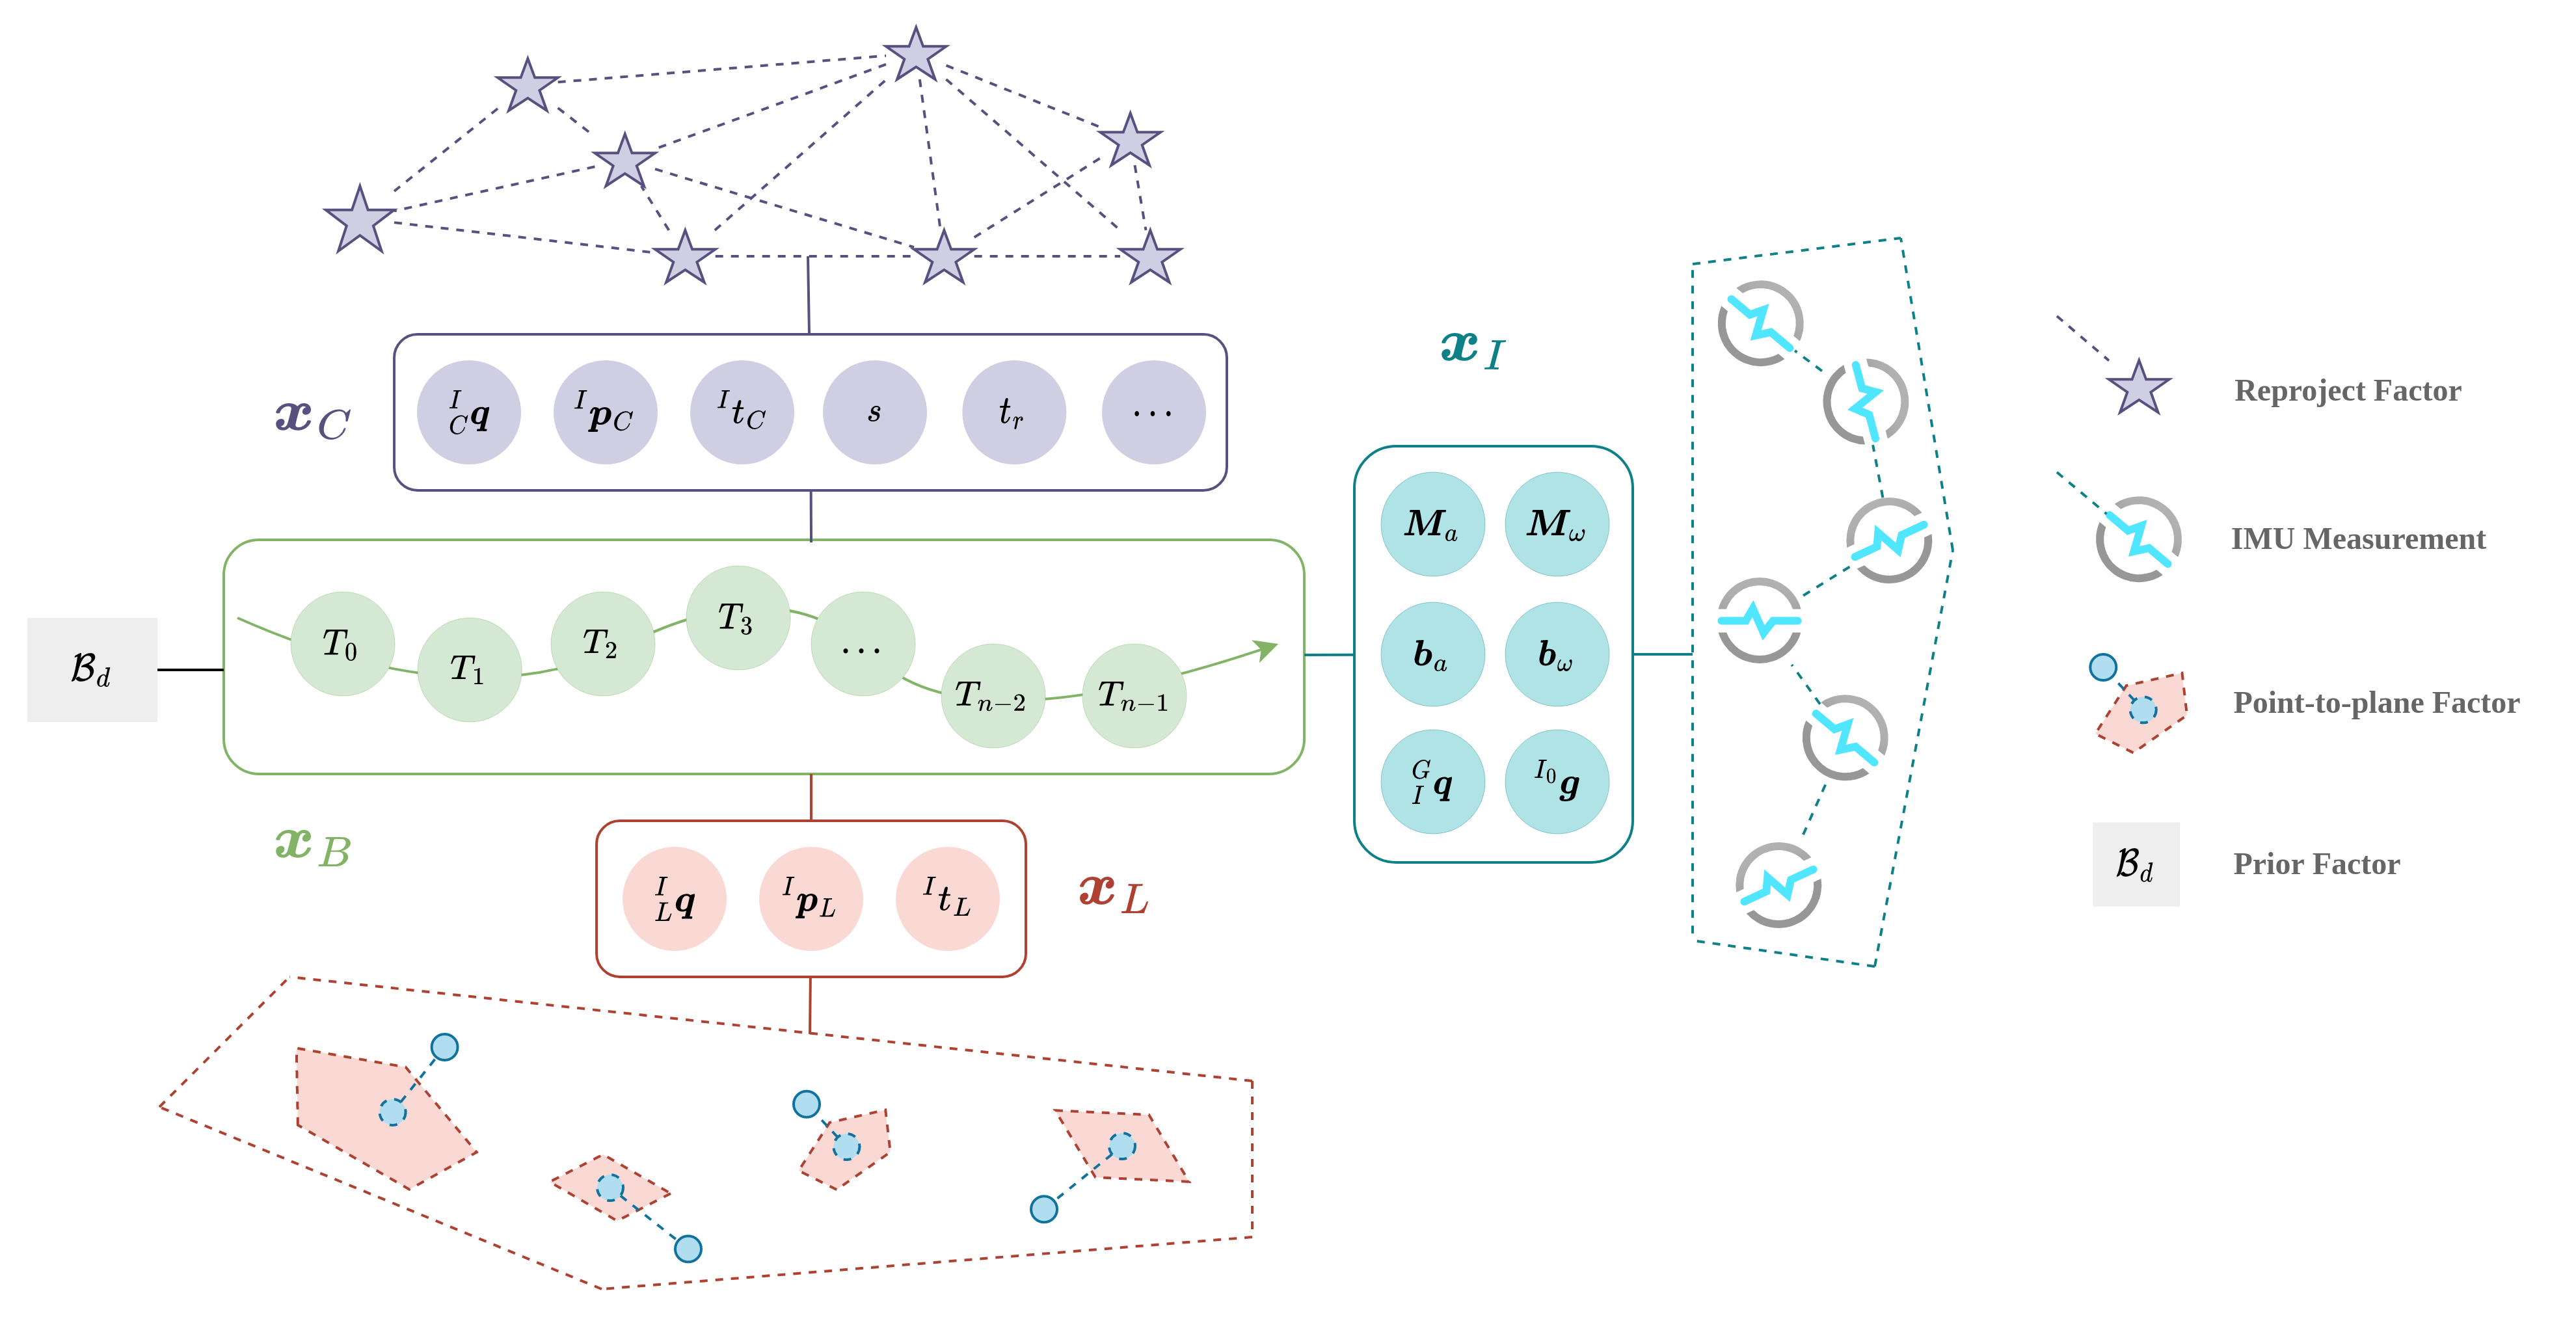
\includegraphics[width=0.9\linewidth]{img/graph.png}
    \caption{\normf{基于连续时间的LiDAR/Camera/IMU的时空标定方法因子图建模}}
    \label{fig:problem_model}
  \end{figure}
}

基于以上的四种因子,最终的图优化问题可以表示为:
\begin{equation}
  \begin{aligned}
     & \min_{\boldsymbol{x}}\left(
    f(\boldsymbol{x}_I,\boldsymbol{x_B}) +
    f(\boldsymbol{x}_L,\boldsymbol{x_B}) +
    f(\boldsymbol{x}_C,\boldsymbol{x_B})
    \right)  \quad\mathrm{s.t.}\quad	\mathcal{B}_d=3                                                                                     \\
     & f(\boldsymbol{x}_I,\boldsymbol{x_B})=\sum_{\mathcal{D}_I}\left( \rho_a\left( \Vert\boldsymbol{r}^i(a)\Vert^2_{\Sigma_a}\right) +
    \rho_\omega\left( \Vert\boldsymbol{r}^i(\omega)\Vert^2_{\Sigma_\omega}\right) \right)                                               \\
     & f(\boldsymbol{x}_L,\boldsymbol{x_B})=\sum_{\mathcal{D}_L}\rho_l\left( \Vert\boldsymbol{r}_{ij}^k(l)\Vert^2_{\Sigma_l}\right)     \\
     & f(\boldsymbol{x}_C,\boldsymbol{x_B})=\sum_{\mathcal{D}_C}\rho_c\left( \Vert\boldsymbol{r}_{ij}^{mn}(c)\Vert^2_{\Sigma_c}\right)
  \end{aligned}
\end{equation}
其中:$\boldsymbol{r}^i(a)$、$\boldsymbol{r}^i(\omega),i\in\mathcal{I}^\dagger$表示基于加速度计和陀螺仪输出信息构建的损失函数,对应的方差矩阵为$\Sigma_a$、$\Sigma_\omega$;$\boldsymbol{r}_{ij}^k(l),i\in\mathcal{E}^\dagger
  ,j\in\mathcal{L}^\dagger,k\in(\mathcal{L}_j)^\dagger$表示基于LiDAR点云信息构建的点到面损失函数,对应的方差矩阵为$\Sigma_l$;$\boldsymbol{r}_{ij}^{mn}(c),i\in\mathcal{C}^\dagger,j\in\mathcal{F}^\dagger,k\in\mathcal{S}^\dagger$表示基于Camera图像信息构建的重投影损失函数,对应的方差矩阵为$\Sigma_c$。另外,在求解该图优化问题时,为了抑制错误关联的干扰(尤其是点到面关联和重投影关联),本文使用了Huber核函数$\rho$对误差$e$进行映射:
\begin{equation}
  \rho(e)=\begin{cases}
    \begin{aligned}
       & \frac{1}{2}e^2\quad                 & \vert e\vert\le\delta \\
       & \vert e\vert-\frac{1}{2}\delta\quad & \vert e\vert>\delta
    \end{aligned}
  \end{cases}
\end{equation}
其中$\delta$为误差阈值:当误差大于$\delta$时,对误差进行线性映射,反之则对误差进行二次曲线映射。